\subsection{Комбинаторные объекты. Коды Грея. Формула включения-исключения. Лемма Бернсайда и Теорема Пойа. Числа Стирлинга. Подсчёт деревьев. Метод производящих функций.}

\subsubsection{Коды Грея}
Код Грея - код для элементов упорядоченного множества (например, чисел от 1 до $n$), такой что расстояние Хэмминга между кодами соседних элементов = 1.
\begin{figure}[H]
	\centering
	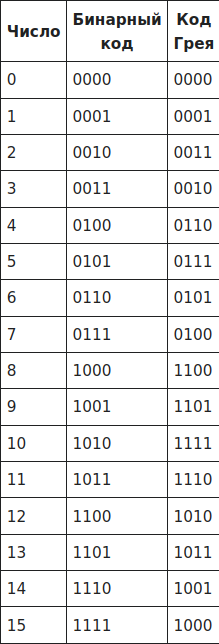
\includegraphics[scale=0.4]{images/grey.png}
\end{figure}

Коды Грея легко получаются из двоичных чисел путём побитовой операции «Исключающее ИЛИ» с тем же числом, сдвинутым вправо на один бит и в котором старший разряд заполняется нулём. Следовательно, $i$-й бит кода Грея $G_i$ выражается через биты двоичного кода $B_i$ следующим образом:
\begin{align*}
G_i = B_i \oplus B_i + 1
\end{align*}

где $\oplus$ — операция «исключающее ИЛИ»; биты нумеруются справа налево, начиная с младшего. 

Декодинг происходит по формуле 
\begin{align*}
	B_i = B_{i + 1} \oplus G_i
\end{align*}

Код Грея назван «рефлексивным» (отражённым) из-за того, что первая половина значений при изменении порядка эквивалентна второй половине, за исключением старшего бита. Старший бит просто инвертируется. При делении каждой новой половины пополам это свойство сохраняется.

Код Грея используется в тех случаях, когда мы медленно считываем значения, а они меняются. Представим себе, что код (обычный двоичный) перескакивает $3\rightarrow4$, или $011_2 \rightarrow 100_2$. Если из-за несовершенства считывателя мы прочитаем первый бит от $011$, а остальные два — от $100$, мы получим $000_2=0$ — число, далёкое от реальных значений. В коде Грея никаких посторонних значений не будет: перескок будет в одном разряде, $010_G \rightarrow 110_G$, и мы считаем либо старое $010_G=3$, либо новое $110_G=4$. 

\subsubsection{Формула включения-исключения}

\T{
	Пусть $A = \bigcup\limits_{i = 1}^nA_i$, тогда по формуле включения-исключения:
	\begin{align*}
		|A| = \sum\limits_{I \in 2^n - 1}(-1)^{|I| + 1}|\bigcap_{j\in I}A_j|
	\end{align*}

	где $N = \{1, \ldots n\}$, $2^N - 1$ - множество всех непустых подмножеств $N$. 
}
\begin{proof}
	\href{https://neerc.ifmo.ru/wiki/index.php?title=%D0%A4%D0%BE%D1%80%D0%BC%D1%83%D0%BB%D0%B0_%D0%B2%D0%BA%D0%BB%D1%8E%D1%87%D0%B5%D0%BD%D0%B8%D1%8F-%D0%B8%D1%81%D0%BA%D0%BB%D1%8E%D1%87%D0%B5%D0%BD%D0%B8%D1%8F}{Доказательство}.
\end{proof}

Формулу включений исключений можно интерпретировать в вероятностном смысле, нужно лишь заменить множества на события, а мощности на вероятности. 

\subsubsection{Лемма Бернсайда}
Я чета в ахуе немного, это из теории групп. Про орбиты. 

\D{
	Говорят, что группа $G$ действует на множестве $M$ слева, если задано отображение $G \times M \rightarrow M$, такое что
	\begin{enumerate}
		\item $g(hm) = (gh)m$ для всех $g, h \in G, m \in M$
		\item $em = m$, где $e$ - нейтральный элемент $G$
	\end{enumerate}
}

\D{
	Подмножество
	\begin{align*}
		Gm = \{gm \mid g \in G\} \subset M
	\end{align*}

	Называется орбитой элемента $m$
}

\T[Лемма Бернсайда]{
	Пусть $G$ — конечная группа, действующая на множестве $X$. Тогда число орбит действия равно среднему количеству точек, фиксированных точек в $X$ элементами $G$.
	
	Точнее, для любого элемента $g \in G$ будем обозначать через $X^g$ множество элементов $X$, оставляемых на месте $g$, то есть
	\begin{align*}
		X^g = \{x \in X \mid gx = x\}
	\end{align*} 

	Тогда
	\begin{align*}
		|X/G| = \frac{1}{|G|}\sum\limits_{g \in G}|X^g|
	\end{align*}
	
	где $|X/G|$ - обозначает число орбит действия.
}
\begin{proof}
	\href{https://neerc.ifmo.ru/wiki/index.php?title=%D0%9B%D0%B5%D0%BC%D0%BC%D0%B0_%D0%91%D1%91%D1%80%D0%BD%D1%81%D0%B0%D0%B9%D0%B4%D0%B0_%D0%B8_%D0%A2%D0%B5%D0%BE%D1%80%D0%B5%D0%BC%D0%B0_%D0%9F%D0%BE%D0%B9%D0%B0#.D0.A2.D0.B5.D0.BE.D1.80.D0.B5.D0.BC.D0.B0_.D0.9F.D0.BE.D0.B9.D0.B0}{Доказательство}.
\end{proof}


\subsubsection{Теорема Пойа}
\href{https://e-maxx.ru/algo/burnside_polya}{Тут} максимально просто написано и про Пойа и про Бернсайда.

\subsubsection{Числа Стирлинга}
\begin{itemize}
	\item \textit{Первого рода.} Количество перестановок из $n$ элементов с $k$ циклами.
	
	Можно посчитать рекурсивно:
	\begin{align*}
		c(n, k) = c(n - 1, k - 1) + (n - 1)\cdot c(n - 1, k)
	\end{align*} 
	\item \textit{Второго рода.} Количество неупорядоченных разбиений $n$-элементного множества на $k$ непустых подмножеств.
	
	Можно посчитать рекурсивно:
	\begin{align*}
		S(n, k) = S(n - 1, k - 1) + k\cdot S(n - 1, k)
	\end{align*}
	
	Есть явная формула:
	\begin{align*}
		S(n, k) = \frac{1}{k!}\sum\limits(-1)^{k + j}{k \choose j}j^n
	\end{align*}
\end{itemize}

\subsubsection{Подсчет деревьев}
\D{
	$n$-ое число Каталана:
	\begin{align*}
		C_n = \frac{1}{n + 1}\binom{2n}{n}
	\end{align*}

	Числа Каталана - удовлетворяют рекуррентному соотношению
	\begin{align*}
		C_0 = 1\\
		C_n = \sum\limits_{i =0}^{n - 1}C_iC_{n - 1 - i}
	\end{align*}
	Например, это количество правильных скобочных последовательностей длины $2n$.
}

Более подробно на \href{https://ru.wikipedia.org/wiki/%D0%A7%D0%B8%D1%81%D0%BB%D0%B0_%D0%9A%D0%B0%D1%82%D0%B0%D0%BB%D0%B0%D0%BD%D0%B0}{Вики}.

\T{
	Количество неизоморфных упорядоченных бинарных деревьев с корнем и $n + 1$ листьями = $n$-ому числу Каталана. 
	
	Здесь \textit{упорядоченные} означает, что ребра, выходящие из каждой вершины, упорядочены.
}

\D{
	Помеченное дерево c $n$ вершинами - дерево c $n$ вершинами, вершинам которого взаимно однозначно соответствуют числа от 1 до $n$.
}

\T[Кэли]{
	Число помеченных деревьев с $n$ вершинами равняется $n^{n - 2}$.
}
\begin{proof}
	Доказательство и еще много всего интересного смотри \href{https://neerc.ifmo.ru/wiki/index.php?title=%D0%9F%D0%BE%D0%B4%D1%81%D1%87%D0%B5%D1%82_%D0%B4%D0%B5%D1%80%D0%B5%D0%B2%D1%8C%D0%B5%D0%B2}{тут}. 
\end{proof}

\subsubsection{Метод производящих функций}
Вот \href{https://neerc.ifmo.ru/wiki/index.php?title=%D0%9F%D1%80%D0%BE%D0%B8%D0%B7%D0%B2%D0%BE%D0%B4%D1%8F%D1%89%D0%B0%D1%8F_%D1%84%D1%83%D0%BD%D0%BA%D1%86%D0%B8%D1%8F}{отсюда} можно прочитать определение и пример для решения рекуррент
